% ============================================================================
\section{Introduction and overview}
% ============================================================================

\begin{frame}{The power of human voice}
  \begin{quote}
    ``Words mean more than what is set down on paper.\\
    It takes the human voice to infuse them with shades of deeper meaning.''
    \begin{flushright}
      --- Maya Angelou, \textit{I Know Why the Caged Bird Sings}
    \end{flushright}
  \end{quote}
\end{frame}

\begin{frame}{A decade of voice technology in products}
  \centering
  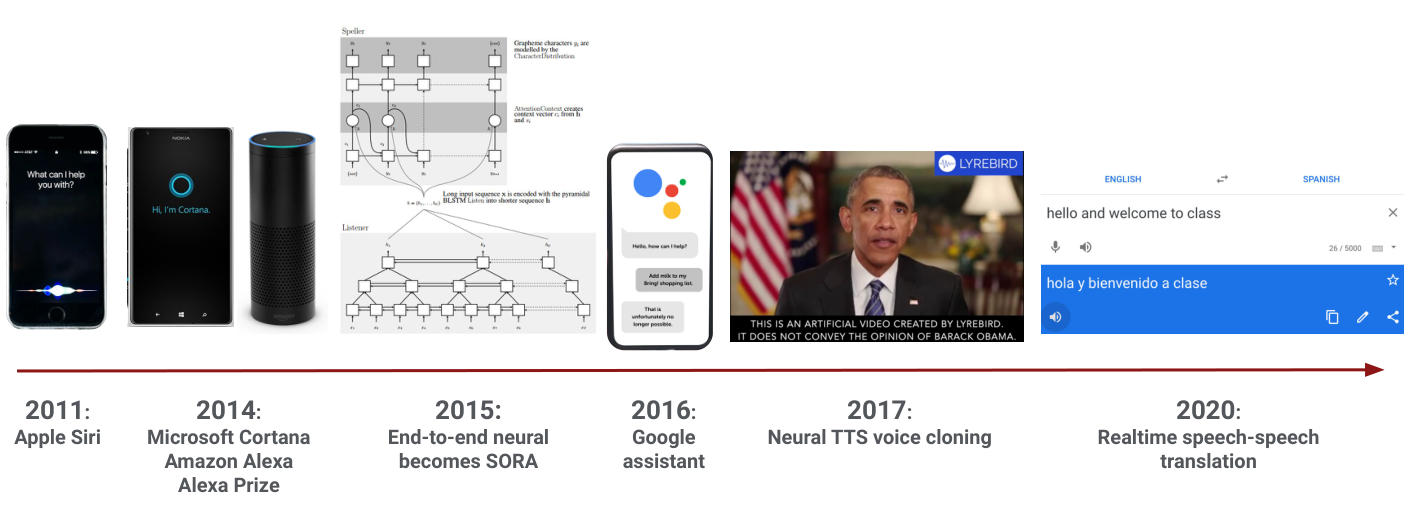
\includegraphics[width=\textwidth,height=0.78\textheight,keepaspectratio]{images/tts/tts_history_timeline.png}
  \slideimgsource{Stanford CS224S, Lecture 1 (2024 Spring), slide 4. The 2015 label is a typo for SOTA, state of the art.}
\end{frame}

\begin{frame}{Where TTS sits: the spoken dialogue pipeline}
  \begin{itemize}\footnotesize
    \item A task-oriented dialogue system recognizes speech, tracks what the user wants, decides what to say, and speaks the answer. TTS is the last stage, and the only one the user actually hears.
  \end{itemize}
  \centering
  
\includegraphics[width=0.92\textwidth,height=0.52\textheight,keepaspectratio]{images/tts/cs224s_compound_ai_pipeline.png}
  \slideimgsource{Architecture of a dialogue-state system for task-oriented dialogue, after Williams et al.\ (2016); Stanford CS224S, Lecture 1 (2024 Spring), slide 19.}
\end{frame}

\begin{frame}{What is Text-to-Speech (TTS)?}
  \begin{itemize}
    \item \textbf{What:} Produce speech from a text input (\textbf{Input:} text, optionally with speaker, language, style, or acoustic prompt; \textbf{Output:} waveform or codec tokens perceived as speech).
    \item \textbf{Applications:}
      \begin{itemize}
        \item Accessibility (screen readers, assistive tech)
        \item Personal Assistants (Apple Siri, Microsoft Cortana, Google Assistant)
        \item Navigation, games, announcements/voice-overs, audiobooks, dubbing, AR/VR
        \item Synthetic data for ASR
      \end{itemize}
    \end{itemize}
\end{frame}

\begin{frame}{What is Text-to-Speech (TTS)?}
  \begin{itemize}
    \item \textbf{Core difficulty:} Many-to-many mapping: the same text admits many natural realizations (prosody, rate, emphasis).
    \item \textbf{New variation:} Voice cloning: TTS systems that mimic particular speakers with minimal training data.
  \end{itemize}
\end{frame}

\begin{frame}{Prosody: Why the Same Text Sounds Different}
  \begin{itemize}
    \item \textbf{Prosody} covers everything the words alone do not fix: intonation (the pitch contour, $F_0$), duration and rhythm, and energy (stress).
    \item Stress changes meaning: ``\textbf{I} never said she stole my money'' accuses differently than ``I never said she stole \textbf{my} money''. Seven words, seven readings, one spelling.
    \item Intonation signals sentence type: statements tend to fall in pitch, yes/no questions tend to rise.
    \item TTS systems model prosody implicitly (attention, latent variables) or explicitly (FastSpeech~2 predicts duration, pitch, and energy per phoneme).
  \end{itemize}
\end{frame}

\begin{frame}{TTS Overview}
  \begin{itemize}
    \item Collect lots of speech (5--50 hours) from one speaker, transcribed carefully down to syllables and phones.
    \item Rapid recent progress in neural approaches.
    \item Modern systems are DNN-based, understandable, but not yet fully emotive.
    \item No longer require extensive data from a single speaker to make a TTS voice for them.
  \end{itemize}
\end{frame}

\begin{frame}{TTS: Definitions}
  \begin{itemize}
    \item \textbf{Codec:} A coder/decoder system that encodes analog speech signals into a digitized, discrete compressed representation for compression.
    \item The discrete symbols a codec produces as its compressed form can serve as \textbf{discrete codes} for language modeling.
    \item A codec typically consists of:
      \begin{itemize}
        \item An \textbf{encoder} (\textit{e.g.}, convnets) that downsamples speech into an embedding,
        \item A \textbf{quantizer} that converts the embedding into a series of discrete tokens,
        \item A \textbf{decoder} (\textit{e.g.}, convnets) that upsamples the tokens/embedding back into a (lossy) reconstructed waveform.
      \end{itemize}
  \end{itemize}
\end{frame}

\begin{frame}{TTS: Modular Pipeline}
  \begin{enumerate}
    \item \textbf{Text analysis:} normalization, tokenization, G2P
    \item \textbf{Acoustic model:} mel, latents, or codec codes over time
    \item \textbf{Vocoder / decoder:} waveform or neural codec inversion
  \end{enumerate}
  \centering
  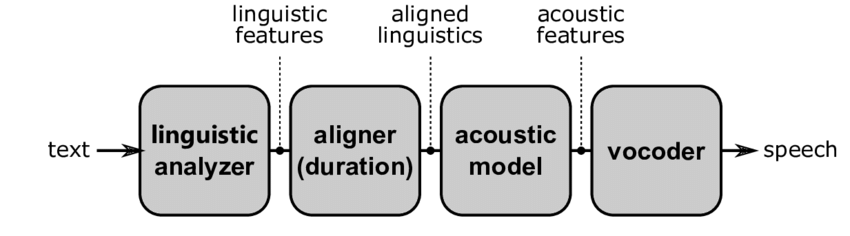
\includegraphics[width=0.86\textwidth,height=0.5\textheight,keepaspectratio]{images/audio-nlp/tts_pipeline.png}
  \slideimgsource{H.-T.~Luong, ``Deep learning based voice cloning framework for a unified system of text-to-speech and voice conversion,'' PhD thesis, SOKENDAI, 2020, Fig.~2.1.}
\end{frame}

\begin{frame}{Three eras of text-to-speech}
  \begin{itemize}
    \item \textbf{Pre-2016:} concatenative unit selection and statistical parametric (HMM/GMM) synthesis.
    \item \textbf{2016--2021:} neural end-to-end models (Tacotron~2, WaveNet vocoders, FastSpeech, Glow-TTS, VITS).
    \item \textbf{2022--present:} diffusion, flow matching, and \textbf{foundation audio} models (VALL-E, Voicebox) with zero-shot cloning and in-context control.
    \item Each era targets bottlenecks of the previous one: flexibility, fidelity, latency, then controllability at scale.
  \end{itemize}
\end{frame}

\begin{frame}{Three eras of text-to-speech}
  \footnotesize
  {\scriptsize
  \begin{tabular}{@{}llll@{}}
    \hline
    \textbf{Era} & \textbf{Technology} & \textbf{Strength} & \textbf{Bottleneck} \\
    \hline
    Concatenative & Unit / diphone selection & Local timbre & Huge DB; brittle joins \\
    Statistical (SPSS) & HMM / GMM vocoder params & Small footprint; adaptation & Muffled, averaged sound \\
    Neural (E2E) & Tacotron~2 + neural vocoder & High fidelity; simpler stack & Slow AR inference \\
    Foundation & VALL-E, Voicebox & Zero-shot; in-context learning & Data scale; misuse risk \\
    \hline
  \end{tabular}
  }
\end{frame}
